% Build me with pdflatex, then use pdf2svg to convert me to an svg file that can go into the repo!

\documentclass[crop, tikz]{standalone}

\usepackage[utf8]{inputenc}

\usepackage{xcolor}

\usetikzlibrary{backgrounds}

\newcommand{\tab}{
    \hspace{8mm}\nobreakspace\ignorespaces
}

\newcommand{\keyword}[1]{
    \textcolor{black!55!green}{\textbf{#1}}\ignorespaces
}

\newcommand{\funcname}[1]{
    \textcolor{blue}{#1}\ignorespaces
}

\newcommand{\pythonmathtimes}{
    \textcolor{blue!55!red}{*}\ignorespaces
}

\newcommand{\pythoncomment}[1]{
    \textcolor{gray!85!blue}{#1}
}

\begin{document}

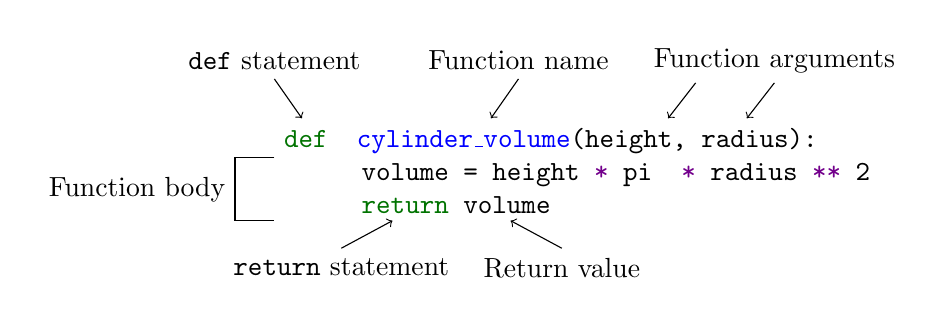
\begin{tikzpicture}[background rectangle/.style={fill=white}, show background rectangle]
    \node[anchor=north west, align=left, font=\tt] at (0,0) {
        \keyword{def}\nobreakspace\funcname{cylinder\_volume}(height, radius):\\
        \tab volume = height\pythonmathtimes\nobreakspace pi \pythonmathtimes\nobreakspace radius\pythonmathtimes\pythonmathtimes\nobreakspace2\\
        \tab\keyword{return}\nobreakspace volume
    };

    % Labels for components of function
    % function definition
    \draw[<-] (0.35,0) -- (0,0.5) node[anchor=south] {{\tt def} statement};
    \draw[<-] (2.75,0) -- (3.1, 0.5) node[anchor=south] {Function name};
    \draw[<-] (6,0) -- (6.35, 0.45) node[anchor=south] {Function arguments};
    \draw[<-] (5,0) -- (5.35, 0.45);
    % body of the function
    \draw[black] (0,-0.5) -- (-0.5,-0.5) -- (-0.5,-1.3) -- (0,-1.3);
    \node[anchor=east] at (-0.5,-0.9) {Function body};
    % return statement
    \draw[<-] (1.50,-1.3) -- (0.85,-1.65) node[anchor=north]{{\tt return} statement};
    \draw[<-] (3,-1.3) -- (3.65,-1.65) node[anchor=north] {Return value};
\end{tikzpicture}

\end{document}
